{\raggedright
\subsection{Introducción general de los Sistemas Distribuidos}
}

En años recientes, el avance en las tecnologías de cómputo y las telecomunicaciones han permitido una gran expansión de los sistemas de información, así como su alta disponibilidad, independientemente de su campo de aplicación.

Las telecomunicaciones permiten la conectividad de un gran número de usuarios ubicados en cualquier parte del mundo por medio de la transmisión de voz, datos o video a través de una gran variedad de dispositivos. Diferentes redes de comunicación de área local (LAN), metropolitanas (MAN), así como de área amplia (WAN), pueden ser accedidas a través de Internet. Esto ha permitido que paralelamente surjan instalaciones de cómputo donde pueden ser desplegadas aplicaciones para realizar procesamiento distribuido de tareas. Estas nuevas facilidades ofrecen a los usuarios y organizaciones una gran flexibilidad para estructurar sus propios sistemas de información de una manera eficiente, así como la oportunidad de interactuar con otros sistemas de información de una manera distribuida. Como consecuencia, esto ha generado una gran dependencia de estos sistemas distribuidos para poder transmitir o procesar información.

Tanenbaum define un sistema distribuido como una colección de computadoras independientes que aparecen ante los usuarios del sistema como una única computadora. El advenimiento de los sistemas distribuidos ha estado soportado en dos importantes innovaciones tecnológicas.

\begin{center}
\section{Unidad I. Introducción a la computación distribuida.}
\end{center}

Sistema Distribuido: Conjunto de computadoras que se interconectan en red para colaborar entre sí y realizar una tarea conjunta como si la realizara un solo computador.

\begin{figure}[h!]
		\centering
		{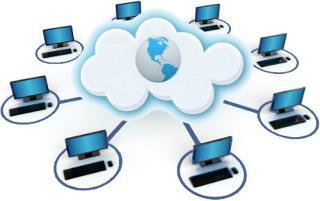
\includegraphics[scale=.5]{1.jpg}\par} \vspace{1cm}
\end{figure}

Los sistemas distribuidos se implementan en diversas plataformas de hardware. Sus componentes de Hw y Sw no comparten un espacio de memoria común, debido a ello se deben coordinar mediante el paso de mensajes.

\begin{figure}[h!]
		\centering
		{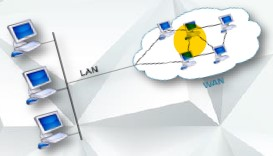
\includegraphics[scale=.7]{2.jpg}\par} \vspace{1cm}
\end{figure}

{\raggedright
\subsection{Características}
}

\begin{itemize}
	\item Transparencia
	\item Consistencia
	\item Flexibilidad
	\item Funcionalidad
	\item Seguridad
	\item Confiabilidad
	\item Repartición carga
	\item Desempeño
	\item Escalabilidad
\end{itemize}

\textbf{Transparencia}: Característica para ocultar el funcionamiento del sistema y su construcción como, por ejemplo:

\begin{itemize}
	\item Trasparencia de localización
	\item Transparencia de migración
	\item Transparencia de réplica
	\item Transparencia de concurrencia
	\item Transparencia de paralelismo
	\item Transparencia de fallas
	\item Transparencia de desempeño
	\item Transparencia de escalabilidad
	\begin{figure}[h!]
		\centering
		{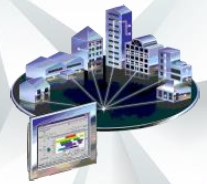
\includegraphics[scale=1]{3.jpg}\par} \vspace{1cm}
	\end{figure}
\end{itemize}

{\raggedright
Tipos de transparencia
}

1. \textbf{Localización}: Ocultar la localización de los datos

2. \textbf{Migración}: Los recursos se pueden mover sin cambiar su nombre

3. \textbf{Replica}: Ocultar el número de copias existentes

4. \textbf{Concurrencia}: Varios usuarios pueden compartir recursos de manera automática

5. \textbf{Paralelismo}: Paralelismo sin que el usuario lo perciba

6. \textbf{Fallas}: Cuando una computadora del sistema falla, esta es imperceptible para el usuario

7. \textbf{Desempeño}: El funcionamiento y velocidad de las máquinas

8. \textbf{Escalabilidad}: El usuario ignora cuándo en el sistema agrega otra computadora

\vspace{1cm}

\textbf{Mantenimiento de consistencia}: Revisión del funcionamiento con el sistema operativo dentro de un sistema distribuido, algunas cosas a considerar son:

\begin{itemize}
	\item Cache
	\item Fallas
	\item Replicación
	\item Interfaz de usuario
	\item Reloj
\end{itemize}

\textbf{Flexibilidad}: Facilita modificaciones al diseño inicial.\hfill \break

\textbf{Funcionalidad}: El sistema distribuido debe funcionar bajo su régimen y debe ser más eficiente que un sistema centralizado...\hfill \break

\textbf{Confiabilidad}: En caso de que una computadora falle, otra la pueda sustituir en la realización de sus tareas asignadas.\hfill \break

\textbf{Repartición de la carga}: Análisis de los equipos del sistema y sus diferentes recursos de cómputo.\hfill \break

\textbf{Desempeño}: Tiempos de respuesta de una aplicación.\hfill \break

\textbf{Escalabilidad}: Permite que a la arquitectura actual se le pueda adicionar más poder de cómputo.

\begin{center}
\subsection{Tipos de modelos de sistemas}
\end{center}

\textbullet{} \textbf{Servidores estación de trabajo }\textbf: Estaciones de trabajo dispersas en un edificio o campus, conectadas entre sí por una red LAN de alta velocidad. Estaciones de trabajo pueden tener discos locales o estaciones sin disco. Las estaciones cuentan con un servidor de archivos.

{\raggedright

\vspace{3pt} \noindent
\begin{tabular}{|p{120pt}|p{120pt}|p{141pt}|}
\hline
\parbox{120pt}{\centering 
\textbf{Uso del disco}
} & \parbox{120pt}{\centering 
\textbf{Ventajas}
} & \parbox{141pt}{\centering 
\textbf{Desventajas}
} \\
\hline
\parbox{120pt}{\centering 
{\small Sin disco}
} & \parbox{120pt}{\centering 
{\small Bajo costo, fácil mantenimiento del Hw. Y SW. Simetría y flexibilidad}
} & \parbox{141pt}{\centering 
{\small Gran uso de la red, los servidores de archivos se pueden convertir en cuellos de botella}
} \\
\hline
\parbox{120pt}{\centering 
{\small Paginación, archivos de tipo borrador}
} & \parbox{120pt}{\centering 
{\small Reduce la carga de la red comparado con el caso sin discos}
} & \parbox{141pt}{\centering 
{\small Un costo alto debido al gran número de discos necesarios}
} \\
\hline
\parbox{120pt}{\centering 
{\small Paginación, archivos de tipo borrador, binarios}
} & \parbox{120pt}{\centering 
{\small Reduce todavía más la carga sobre la red}
} & \parbox{141pt}{\centering 
{\small Altos costo, complejidad adicional para actualizar los binarios}
} \\
\hline
\parbox{120pt}{\centering 
{\small Paginación, archivos de tipo borrador, ocultamiento de archivos}
} & \parbox{120pt}{\centering 
{\small Una carga aún menor en la red, también se reduce la carga en los servidores de archivos}
} & \parbox{141pt}{\centering 
{\small Alto costo, problema de consistencia del caché}
} \\
\hline
\parbox{120pt}{\centering 
{\small Sistema local de archivos completo}
} & \parbox{120pt}{\centering 
{\small Escasa carga en la red, elimina la necesidad de los servidores de archivos}
} & \parbox{141pt}{\centering 
{\small Perdida de transparencia}
} \\
\hline
\end{tabular}
\vspace{2pt}

}
\vspace{1.5cm}
\textbullet{} \textbf{Pila de procesadores}: Consiste en un conjunto de procesadores, los cuales se pueden asignar dinámicamente a los usuarios según la demanda.

Los usuarios no disponen de estaciones de trabajo personales, en este modelo se les dan terminales gráficas de alto rendimiento, no se tiene la propiedad de los procesadores debido a que pertenecen a todos compartida mente y un servidor de archivos.

\begin{figure}[h!]
		\centering
		{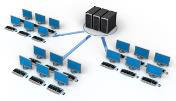
\includegraphics[scale=.7]{4.jpg}\par} \vspace{1cm}
\end{figure}

{\raggedright
\textbullet{} \textbf{Multiprocesadores con memoria compartida y con memoria distribuida}: Taxonomía es la clasificación de las distintas arquitecturas de computadoras.
}

\begin{center}
Clasificación de Flynn:
\end{center}

\begin{itemize}
	\item SISD
	\item SIMD
	\item MISD
	\item MIMD
\end{itemize}

La taxonomía de Flynn es la clásica clasificación usada en computación paralela, la cual usa ideas familiares al campo de la computación convencional para proponer una taxonomía de arquitecturas de computadores.

{\raggedright
\subsubsection{\textbf{SISD}}
}

Se refiere a las computadoras convencionales de Von Neumann. Son equipos con un solo procesador que trabaja sobre un solo dato a la vez. A estos equipos se les llama también computadoras secuenciales.

Todas las computadoras SISD utilizan un registro simple llamado: el contador del programa, el cual lleva el conteo de la ejecución serial de las instrucciones.

\vspace{1cm}
\begin{center}
Características SISD
\end{center}

\begin{itemize}
	\item Flujo único de instrucciones.
	\item Flujo único de datos.
	\item Corresponde al modelo estructural básico, con un procesador de instrucciones y un procesador de datos.
	\item Tiene una única vía de acceso a la memoria principal.
	\item Este es el modelo tradicional de computación secuencial donde una unidad de procesamiento recibe una sola secuencia de instrucciones que operan en una secuencia de datos.
\end{itemize}

\begin{center}
Diagrama SISD
\end{center}

\begin{figure}[h!]
		\centering
		{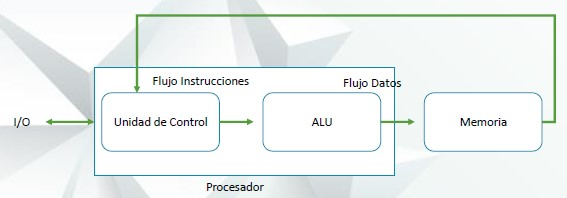
\includegraphics[scale=1]{5.jpg}\par} \vspace{1cm}
\end{figure}

\begin{center}
Ventajas y desventajas de SISD
\end{center}

{\raggedright
\textbf{Ventajas}:
}

\begin{itemize}
	\item Requiere menos energía.
	\item No se tiene un protocolo de comunicación complejo.
	\item Los datos en cuestión se almacenan en una única memoria en la cual se usan técnicas como la segmentación para evitar errores de fragmentación interna.
\end{itemize}

{\raggedright
\textbf{Desventajas}:
}

\begin{itemize}
	\item Velocidad limitada.
	\item No es útil para aplicaciones amplias.
\end{itemize}

{\raggedright
\subsubsection{\textbf{SIMD}}
}

Este tipo de sistemas tienen múltiples flujos de datos entrantes y un número de unidades de procesamiento que pueden actuar sobre una sola instrucción en cualquier momento.

Su funcionamiento es el siguiente un simple controlador envía las instrucciones, una a una, a un arreglo de procesadores que operan en el esquema maestro esclavo. Es decir, las instrucciones son difundidas desde la memoria a un conjunto de procesadores. Así, cada procesador es simplemente una unidad aritmética lógica y se tiene una sola unidad de control Todos los procesadores ejecutan cada operación recibida al mismo tiempo, por lo cual, cada uno ejecuta la misma instrucción sobre diferentes datos.
\vspace{1cm}
\begin{center}
Diagrama SIMD
\end{center}

\begin{figure}[h!]
		\centering
		{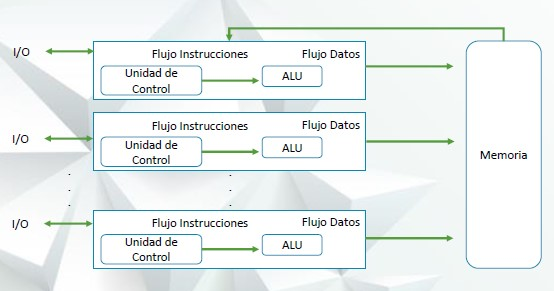
\includegraphics[scale=.7]{6.jpg}\par} \vspace{1cm}
\end{figure}

\begin{center}
Ventajas y desventajas de SIMD
\end{center}

{\raggedright
\textbf{Ventajas}:
}

\begin{itemize}
	\item La misma operación en varios elementos se puede realizar usando una sola instrucción.
	\item El rendimiento del sistema se puede incrementar aumentando el número de núcleos del procesador.
	\item Mayor velocidad de ejecución que SISD.
	\item Útil para distintas áreas como Imágenes.
\end{itemize}

{\raggedright
\textbf{Desventajas}:
}

\begin{itemize}
	\item Existe una comunicación compleja entre el número de núcleos del procesador.
	\item El costo es más alto que la arquitectura SISD.
\end{itemize}

{\raggedright
\subsubsection{\textbf{MISD}}
}

Los sistemas con flujo MISD tienen varias unidades de procesamiento que realizan diferentes operaciones mediante la ejecución de diferentes instrucciones en el mismo conjunto de datos.Implementaciones de esta arquitectura no existen realmente.

La idea es descomponer las unidades de procesamiento en fases, en donde cada una se encarga de una parte de las operaciones a realizar. De esta manera, parte de los datos pueden ser procesados en la fase 1 mientras otros son procesados en la 2 otros en la tres, y así sucesivamente. El flujo de información es continuo y la velocidad de procesamiento crece con las etapas.
\vspace{1cm}
\begin{center}
Diagrama MISD
\end{center}
\begin{figure}[h!]
		\centering
		{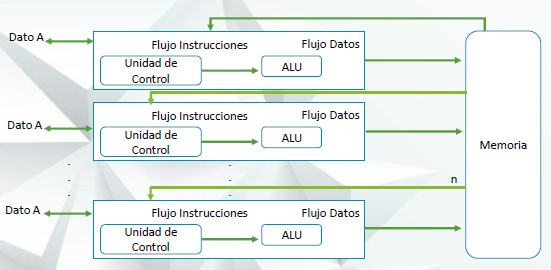
\includegraphics[scale=.7]{7.jpg}\par} \vspace{1cm}
\end{figure}

{\raggedright
\subsubsection{\textbf{MIMD}}
}

En el sistema que usa la arquitectura MIMD, cada procesador en un sistema multiprocesador puede ejecutar diferentes conjuntos de instrucciones de forma independiente en los diferentes conjuntos de datos en paralelo.

Las maquinas MIMD tienen más de un procesador y cada uno puede ejecutar un programa diferente, con múltiples datos. En muchos sistemas cada procesador tiene acceso a una memoria global, para reducir el tiempo de comunicación entre los procesadores. Además, cada procesador tiene una memoria privada.

\vspace{1cm}
\begin{center}
	{\raggedright
	Los sistemas MIMD se pueden clasificar en:
	}
\end{center}

\begin{itemize}
	\item Sistemas de Memoria Compartida.
	\item Sistemas de Memoria Distribuida.
	\item Sistemas de Memoria Compartida Distribuida.
\end{itemize}
\vspace{1cm}

\begin{center}
Diagrama MIMD
\end{center}

\begin{figure}[h!]
		\centering
		{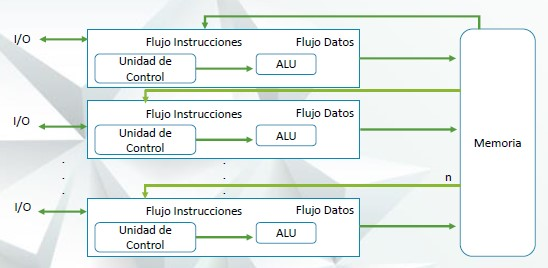
\includegraphics[scale=.7]{8.jpg}\par} \vspace{1cm}
\end{figure}

{\raggedright
\subsection{Actividad 1 en clase}
}

{\raggedright
Desarrolla un código por cada clasificación de Flynn, en el lenguaje de tu preferencia para explicar los multiprocesadores.
}

\begin{figure}[h!]
		\centering
		{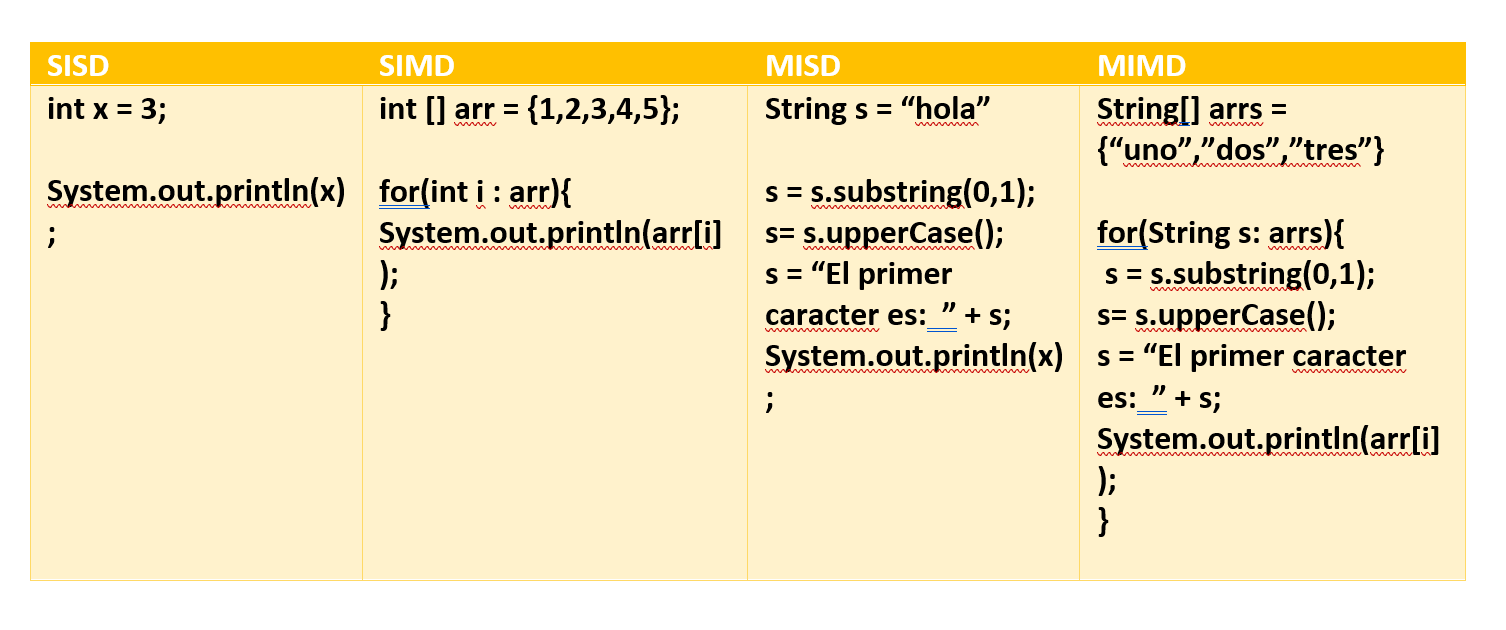
\includegraphics[scale=.5]{9.jpg}\par} \vspace{.5cm}
\end{figure}

{\raggedright
Tipos de memoria en las arquitecturas SIMD y MIMD
}

\begin{itemize}
	\item Sistemas de Memoria Compartida.
	\item Sistemas de Memoria Distribuida.
	\item Sistemas de Memoria Compartida Distribuida.
\end{itemize}

Una clasificación en la cual combinamos los modos de funcionamiento paralelos más comunes de la taxonomía de Flynn (SIMD y MIMD), con los tipos de organización de la memoria (Memoria Compartida (SM) y Memoria Distribuida (DM).

\begin{center}
\subsection{Sistemas de Memoria Compartida}
\end{center}

En este tipo de sistemas cada procesador tiene acceso a toda la memoria, es decir hay un
espacio de direccionamiento compartido. Las computadoras MIMD con memoria compartida son sistemas conocidos como de multiprocesamiento simétrico (SPM) donde múltiples procesadores comparten un mismo sistema operativo y memoria.

\begin{figure}[h!]
		\centering
		{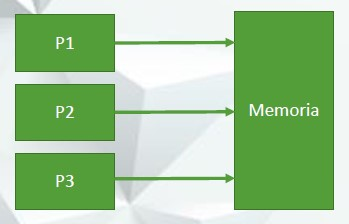
\includegraphics[scale=.7]{10.jpg}\par} \vspace{1cm}
\end{figure}

\begin{center}
\subsection{Sistemas de Memoria Distribuida.}
\end{center}

Estos sistemas tienen su propia memoria local Los procesadores pueden compartir información solamente enviando mensajes. Las computadoras MIMD de memoria distribuida son conocidas como sistemas de procesamiento en paralelo masivo (MPP) donde múltiples procesadores trabajan en diferentes partes de un programa, usando su propio sistema operativo y memoria.

\begin{figure}[h!]
		\centering
		{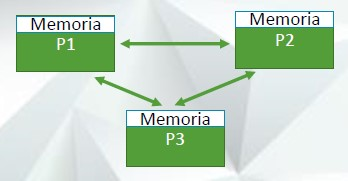
\includegraphics[scale=.7]{11.jpg}\par} \vspace{1cm}
\end{figure}

\begin{center}
Sistemas de Memoria Compartida Distribuida\textbf{{\Large .}}
\end{center}

Es una partición de procesadores que tienen acceso a una memoria compartida común, pero sin un canal compartido Esto es, físicamente cada procesador posee su memoria local y se interconecta con otros procesadores por medio de un dispositivo de alta velocidad, y todos ven las memorias de cada uno como un espacio de direcciones globales.

\begin{figure}[h!]
		\centering
		{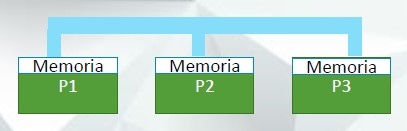
\includegraphics[scale=.7]{12.jpg}\par} \vspace{1cm}
\end{figure}

\begin{center}
\subsubsection{Sistemas con memoria compartida}
\end{center}
\vspace{1cm}

Soporte de Software:

\begin{itemize}
	\item Resuelven problemas de secciones críticas.
	\item Primitivas de sincronización: semáforos, contadores, secuenciadores y monitores.
	\item Comunicación por espacios de memoria compartida.
\end{itemize}
\vspace{1cm}

Soporte de Hardware:

\begin{itemize}
	\item Limitado en la escalabilidad.
	\item Difícil de construir.
	\item El acceso a la memoria es un cuello de botella.
\end{itemize}
\vspace{1cm}

\begin{center}
\subsubsection{Sistemas con memoria distribuida}
\end{center}

Soporte de Software:

\begin{itemize}
	\item Pase de mensajes: Trae complicaciones adicionales como perdida de mensajes, perdida de orden, etc.
	\item Protocolos de comunicación: Buffering y bloqueos
\end{itemize}

Soporte de Hardware:

\begin{itemize}
	\item Fácil de construir
	\item La escalabilidad no está limitada.
\end{itemize}

\begin{center}
\subsection{Taxonomía de los sistemas distribuidos}
\end{center}

\begin{itemize}
	\item Sistemas con software débilmente acoplado en hardware débilmente acoplado NFS (Network File System).
	\item Sistemas con software fuertemente acoplado en hardware fuertemente acoplado; Sistemas operativos de multiprocesador (paralelos).
	\item Sistemas con software fuertemente acoplado en hardware débilmente acoplado; Sistemas realmente distribuidos (imagen de sistema único).
\end{itemize}

\begin{figure}[h!]
		\centering
		{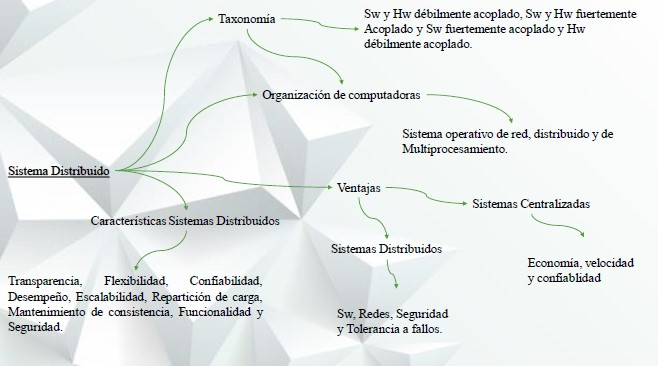
\includegraphics[scale=.9]{13.jpg}\par} \vspace{1cm}
\end{figure}
\newpage

\begin{center}
\section{Redes.}
\end{center}

{\raggedright
\subsection{Actividad 2 en clase.}
}

{\raggedright
Desarrolla una topología de red, explicando cada uno de sus componentes visto en el ejemplo del diagrama.
}

\begin{figure}[h!]
		\centering
		{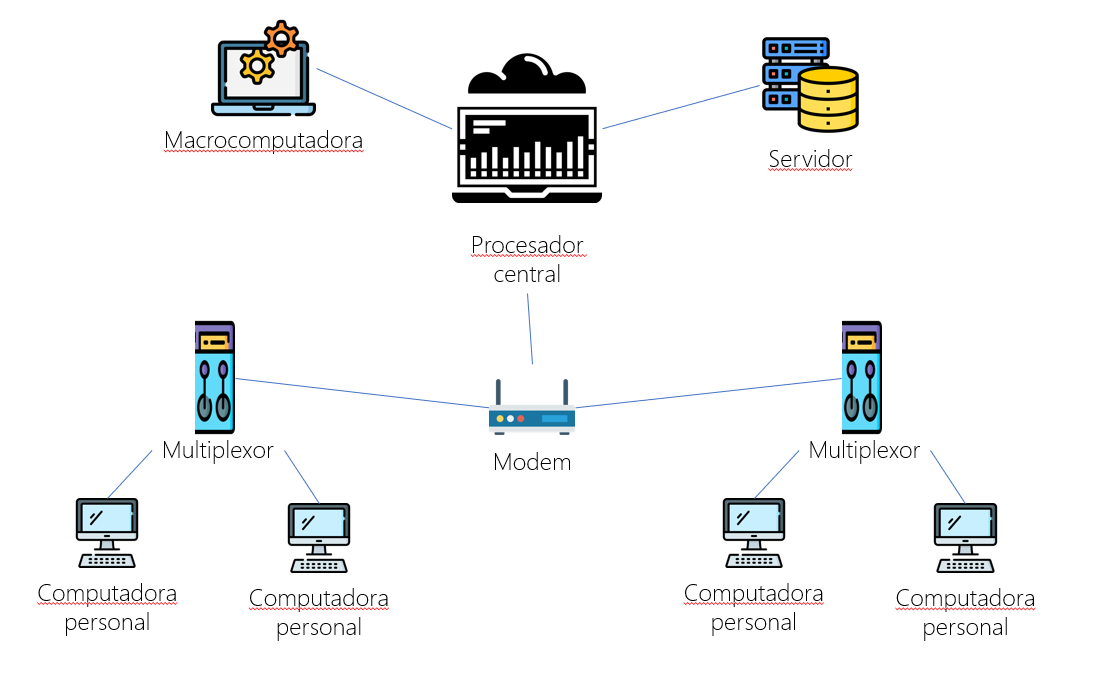
\includegraphics[scale=.4]{14.jpg}\par} \vspace{1cm}
\end{figure}

\begin{center}
\subsection{Principales componentes de una red}
\end{center}

\begin{itemize}
	\item \textbf{Medios de comunicación}: Transportar datos (líneas telefónicas, canal LAN).
	\item \textbf{Macrocomputadoras}: Computadoras donde están las grandes bases de datos en un ambiente centralizado.
	\item \textbf{Terminales de cómputo}: Dispositivos de I/O.
	\item \textbf{Enrutadores}:: Dispositivo que examina las direcciones de la red dentro de un protocolo y encamina paquetes por la ruta.
	\item \textbf{Modem}: Convertir datos digitales seriales a una señal analógica para un canal, y a la Inversa.
	\item \textbf{Multiplexores}: Permite que las terminales compartan la línea de comunicación y reduce el número de líneas usadas.
	\item Estaciones de trabajo
	\item Conmutadores
	\item \textbf{Procesador Central}: Maneja el procesamiento de comunicación entre macrocomputadora y los canales de comunicación.
	\item \textbf{Servidores}: Su propósito es proporcionar rendimiento y servicios a estaciones de trabajo.
\end{itemize}
\vspace{1cm}

\begin{center}
\subsection{Modos de operación y conmutación}
\end{center}

Modos para trasmitir datos por un enlace de comunicación:
\begin{itemize}
	\item Comunicación simplex: Cuando los datos viajan en una sola dirección.
	\item Comunicación half duplex: Permite que los datos viajen en dos direcciones, una a la vez.
	\item Comunicación full duplex: Los datos viajan simultáneamente en ambas direcciones.
\end{itemize}
\vspace{1cm}

\begin{center}
\subsection{Conmutación}
\end{center}

Las redes utilizan comunicación conmutada para transferir datos, esto permite que los dispositivos compartir líneas físicas de comunicación.


1. \textbf{Conmutación de circuitos}: Se crea una ruta única e interrumpida entre dos dispositivos que se requieran comunicar, esta ruta no se puede ocupar hasta que se finalice la comunicación.

2. \textbf{Conmutación de mensajes}: No se tiene un establecimiento de la ruta, los bloques de mensajes se almacenan en la central de conmutación y se envían uno a la vez Los bloques no tienen límite de tamaño.

3. \textbf{Conmutación de paquetes}: División de datos en fragmentos llamados paquetes que viajan por múltiples rutas entre distintas computadoras. Los paquetes pueden viajar en ambas direcciones, siempre requieren una dirección destino. En la conmutación no se reserva ancho de banda, se toma conforme se necesite, útil en tráfico interactivo.

4. \textbf{Conmutación hibrida}: Son variantes que existen en la conmutación de circuitos y paquetes, como conmutación por conexión rápida y conmutación por división de tiempo.

\newpage

\begin{center}
\subsection{Topología de redes}
\end{center}

Referencia al arreglo geométrico que tendrán las conexiones entre las computadoras
\begin{itemize}
		\item a) \textbf{Topología estrella}: Todas las computadoras se conectan a una computadora central, esta topología no permite la comunicación directa entre dos computadoras que no sean la central.

		\begin{figure}[h!]
				\centering
				{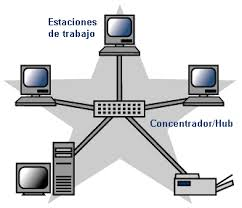
\includegraphics[scale=.3]{15.jpg}\par} \vspace{1cm}
		\end{figure}

		\item b) \textbf{Topología en anillo}: La red forma un anillo continuo en el cual puede viajar la información.
		\begin{figure}[h!]
				\centering
				{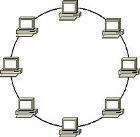
\includegraphics[scale=.7]{16.jpg}\par} \vspace{1cm}
		\end{figure}

		\item c) \textbf{Topología en bus}: Emplea un solo medio llamado bus, al cual todas las computadoras se conectan.
		\begin{figure}[h!]
				\centering
				{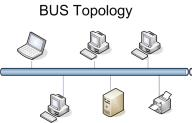
\includegraphics[scale=.7]{17.jpg}\par} \vspace{1cm}
		\end{figure}

		\item d) \textbf{Topología en árbol}: Existe una computadora principal que sirve como raíz y única salida externa.
		\begin{figure}[h!]
				\centering
				{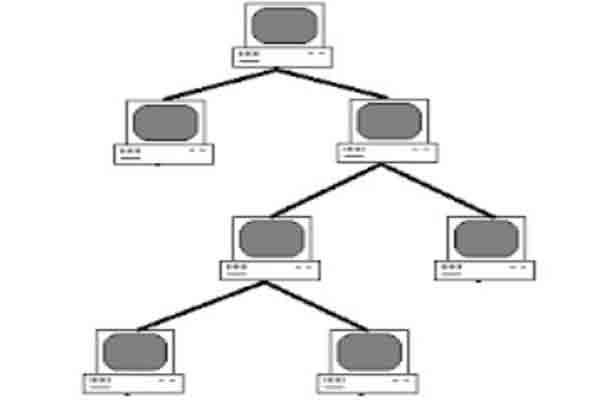
\includegraphics[scale=.15]{18.jpg}\par} \vspace{1cm}
		\end{figure}

		\item e) \textbf{Topología irregular}: No se respeta un modelo de conexión.

		\item f) \textbf{Topología de intersección}: Es esta topología existe la conexión de dos o más tipos de topologías.

		\item g) \textbf{Topología completa}: Se dan todos los tipos de topologías.
		\begin{figure}[h!]
		\centering
		{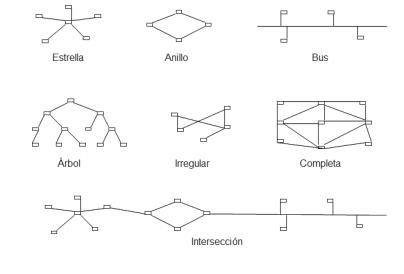
\includegraphics[scale=.7]{19.jpg}\par} \vspace{1cm}
	\end{figure}
\end{itemize}

\begin{center}
\subsection{El procesamiento paralelo}
\end{center}

Sera una forma de multiprocesamiento, es una situación en que dos o más procesadores ejecutan instrucciones de manera simultánea. En sistemas multiprocesamiento, el administrador del procesador debe coordinar la actividad de cada procesador, así como sincronizar la interacción cooperativa entre las CPU.
¿En que nos ayuda un sistema de procesamiento paralelo? Incremento en la confiabilidad y procesamiento más rápido.
\vspace{2.5cm}

\begin{center}
\subsection{Confiabidilad}
\end{center}

Sera la disponibilidad de más de una CPU, si falla un procesador, entonces los otros deben seguir trabajando. Los sistemas paralelos deben diseñarse cuidadosamente de modo que el procesador que fallo pueda informar las fallas y asuman las instrucciones los demás CPU.
En un Sistema paralelo influye mucho el SO. Debido a que el realiza la asignación de recursos de forma que los procesadores restantes no se sobrecarguen.
\vspace{2.5cm}

\begin{center}
\subsection{Velocidad}
\end{center}

Se logra porque algunas veces las instrucciones pueden procesarse en paralelo, dos o más a la vez. En sistemas muy grandes asignan una CPU para un solo programa o trabajo. Otros asignan una CPU a cada conjunto de trabajo o partes de éste. Algunos subdividen las instrucciones individuales de modo que cada subdivisión pueda procesarse de manera simultánea (y tendríamos programación concurrente).\vspace{1.5cm}

\begin{center}
\subsection{Ejemplo real, alusión a paralelismo}
\end{center}

Un restaurante de comida rápida, tiene un sistema multiprocesamiento sincronizado.
\begin{itemize}
	\item Procesador 1 (El que recibe la orden) acepta la solicitud, verifica errores y pasa la solicitud.
	\item Procesador 2 (El empacador) busca la información requerida (i.e. hamburguesa) toma acción a lo que necesita para empacar una hamburguesa.
	\item Procesador 3 (El cocinero) recupera la información de solicitud y toma acción de cocinar la hamburguesa.
	\item Procesador 3 envía al procesador 2 y el procesador 2 realiza las instrucciones de empacar.
	\item Procesador 2 envía a procesador 4 (El cajero).
	\item Procesador 4 envía respuesta del proceso (la orden).
\end{itemize}
Y viene la validación de su sistema, lo que ustedes programan.
El multiprocesamiento va a tener lugar en diferentes niveles, cada nivel se ejerce con una frecuencia de sincronización diferente.


{\raggedright

\vspace{3pt} \noindent
\begin{tabular}{|p{133pt}|p{133pt}|p{133pt}|}
\hline
\parbox{133pt}{\centering 
\textbf{Nivel Paralelismo}
} & \parbox{133pt}{\centering 
\textbf{Procesos}
} & \parbox{133pt}{\centering 
\textbf{Sincronización}
} \\
\hline
\parbox{133pt}{\centering 
Trabajo
} & \parbox{133pt}{\centering 
Cada trabajo tiene su propio procesador y todos los procesos e hilos son ejecutados en el mismo procesador.
} & \parbox{133pt}{\centering 
No se requiere sincronización explicita
} \\
\hline
\parbox{133pt}{\centering 
Proceso
} & \parbox{133pt}{\centering 
Procesos no relacionados, sin importar el trabajo son asignados a cualquier procesador disponible
} & \parbox{133pt}{\centering 
Sincronización moderada para rastrear procesos
} \\
\hline
\parbox{133pt}{\centering 
Hilo
} & \parbox{133pt}{\centering 
Los hilos se asignan a procesadores disponibles.
} & \parbox{133pt}{\centering 
Alto grado de sincronización, y instrucciones explicitas del programador.
} \\
\hline
\end{tabular}
\vspace{2pt}

}

\begin{center}
\subsection{Configuraciones Típicas de multiprocesamiento}
\end{center}

1. Maestro/esclavo.

2. Débilmente acoplada.

3. Simétrica.

1. Es un sistema de multiprocesamiento asimétrico, como si fuera un procesador principal en el sistema. Y tienen procesadores esclavos adicionales. Cada procesador esclavo es comandado por el procesador principal.
Responsable de todos los archivos, dispositivos, memoria y procesadores.

\begin{figure}[h!]
		\centering
		{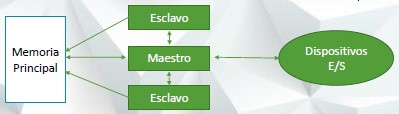
\includegraphics[scale=1]{20.jpg}\par} \vspace{1cm}
\end{figure}

Los procesadores esclavos pueden acceder directamente a la memoria principal, pero deben enviar todas las solicitudes de E/S a través del procesador maestro.\hfill \break

2. Configuración débilmente acoplada.\hfill \break
Cada uno con su propia memoria, dispositivos de E/S, CPU y S.O. Esta configuración se denomina débilmente acoplada porque cada procesador controla sus propios recursos: sus propios archivos. Accesos a la memoria y sus propios dispositivos de E/S, lo cual significa que cada procesador mantiene sus propios comandos y tablas de administración de E/S.
La única diferencia entre un sistema multiprocesamiento y débilmente acoplado y una colección de Sistemas multiprocesamiento independiente es que cada procesador puede comunicarse y cooperar con los otros.

\begin{figure}[h!]
		\centering
		{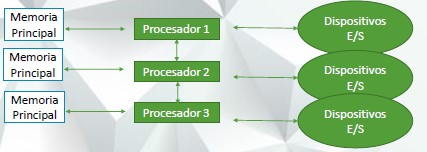
\includegraphics[scale=1]{21.jpg}\par} \vspace{1cm}
\end{figure}

3. Configuración simétrica.\hfill \break
Fuertemente acoplada, es la configuración más difícil de implementar porque los procesos deben estar bien sincronizados para evitar bloqueos. En comparación con una configuración débilmente acoplada, es más confiable, usa los recursos de manera efectiva, puede equilibrar las cargas.

\begin{figure}[h!]
		\centering
		{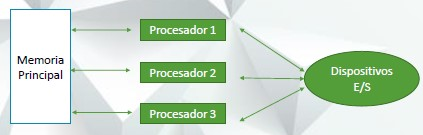
\includegraphics[scale=1]{22.jpg}\par} \vspace{1cm}
\end{figure}


\begin{center}
\subsection{Sincronización}
\end{center}

1. Prueba e inicio.

2. WAIT Y SIGNAL.

3. Semáforos.

\textbf{Prueba e inicio}: : Es una instrucción de máquina única conocida como TS, introducida por IBM para computadoras de un sistema multiprocesamiento 360/370.\hfill \break
Un bit de almacenamiento con cero (libre) o un uno (ocupado), como un subprograma con parámetro de entrada (ubicación de almacenamiento) y retorna un valor (ocupado/libre).\hfill \break
Proceso 1 revisa TS, si está libre entra, de lo contrario espera, es favorable para pocos procesos, pueden llegar varios procesos y esperar esto podría ocasionar inanición (espera indefinida).\hfill \break


\textbf{WAIT Y SIGNAL}: WAIT se activa cuando el proceso se encuentra en condición ocupado, WAIT establece un bloque de control de proceso (PCB) en el estado bloqueado y lo vincula con la cola de los procesos que están esperando entrar.\hfill \break
SIGNAL se activa para revisar a TS si está libre u ocupado, verifica la cola de procesos que están esperando entrar para ser ejecutados, y escoge uno estableciéndolo en estado LISTO.\hfill \break


\textbf{Semáforos}: Un semáforo es una variable entera no negativa, se usa como una señal binaria (bandera). Un semáforo indica cuando está libre un recurso y el proceso puede utilizarlo S= 0 ocupado.
{\raggedright
\vspace{1cm}

\vspace{3pt} \noindent
\begin{tabular}{|p{59pt}p{59pt}p{59pt}p{59pt}p{59pt}p{59pt}|}
\hline
\parbox{59pt}{\centering 
\textbf{Num. Edo}
} & \parbox{59pt}{\centering 
\textbf{Acciones}
} & \parbox{59pt}{\centering 
\textbf{Operación}
} & \parbox{59pt}{\centering 
\textbf{Ejecución}
} & \parbox{59pt}{\centering 
\textbf{Bloqueados}
} & \parbox{59pt}{\centering 
\textbf{Valor S}
} \\
\hline
\parbox{59pt}{\centering 
\textbf{0}
} & \parbox{59pt}{\centering } & \parbox{59pt}{\centering 
libre
} & \parbox{59pt}{\centering } & \parbox{59pt}{\centering } & \parbox{59pt}{\centering 
1
} \\
\hline
\parbox{59pt}{\centering 
\textbf{1}
} & \parbox{59pt}{\centering 
P1
} & \parbox{59pt}{\centering 
ocupado
} & \parbox{59pt}{\centering 
P1
} & \parbox{59pt}{\centering } & \parbox{59pt}{\centering 
0
} \\
\hline
\parbox{59pt}{\centering 
\textbf{2}
} & \parbox{59pt}{\centering 
P1
} & \parbox{59pt}{\centering 
libre
} & \parbox{59pt}{\centering } & \parbox{59pt}{\centering } & \parbox{59pt}{\centering 
1
} \\
\hline
\parbox{59pt}{\centering 
\textbf{3}
} & \parbox{59pt}{\centering 
P2
} & \parbox{59pt}{\centering 
ocupado
} & \parbox{59pt}{\centering 
P2
} & \parbox{59pt}{\centering } & \parbox{59pt}{\centering 
0
} \\
\hline
\parbox{59pt}{\centering 
\textbf{4}
} & \parbox{59pt}{\centering 
P3
} & \parbox{59pt}{\centering 
ocupado
} & \parbox{59pt}{\centering 
P2
} & \parbox{59pt}{\centering 
P3
} & \parbox{59pt}{\centering 
0
} \\
\hline
\parbox{59pt}{\centering 
\textbf{5}
} & \parbox{59pt}{\centering 
P4
} & \parbox{59pt}{\centering 
ocupado
} & \parbox{59pt}{\centering 
P2
} & \parbox{59pt}{\centering 
P3, P4
} & \parbox{59pt}{\centering 
0
} \\
\hline
\parbox{59pt}{\centering 
\textbf{6}
} & \parbox{59pt}{\centering 
P2
} & \parbox{59pt}{\centering 
ocupado
} & \parbox{59pt}{\centering 
P3
} & \parbox{59pt}{\centering 
P4
} & \parbox{59pt}{\centering 
0
} \\
\hline
\parbox{59pt}{\centering 
\textbf{7}
} & \parbox{59pt}{\centering } & \parbox{59pt}{\centering 
ocupado
} & \parbox{59pt}{\centering 
P3
} & \parbox{59pt}{\centering 
P4
} & \parbox{59pt}{\centering 
0
} \\
\hline
\parbox{59pt}{\centering 
\textbf{8}
} & \parbox{59pt}{\centering 
P3
} & \parbox{59pt}{\centering 
ocupado
} & \parbox{59pt}{\centering 
P4
} & \parbox{59pt}{\centering } & \parbox{59pt}{\centering 
0
} \\
\hline
\parbox{59pt}{\centering 
\textbf{9}
} & \parbox{59pt}{\centering 
P4
} & \parbox{59pt}{\centering 
libre
} & \parbox{59pt}{\centering } & \parbox{59pt}{\centering } & \parbox{59pt}{\centering 
1
} \\
\hline
\end{tabular}
\vspace{2pt}

}
\vspace{1cm}

\textbf{Paralelismo explícito}: Plantear explícitamente cuales instrucciones pueden ejecutarse en paralelo.

\textbf{Paralelismo implícito}: Detección automática por el compilador de instrucciones que pueden realizarse en paralelo. \hfill \break

\begin{center}
Ejemplo1: \textbf{A=3*B*C+4/(D+E)*(F-G)}
\end{center}

\begin{center}
\textbf{Secuencial}
\end{center}

{\raggedright

\vspace{3pt} \noindent
\begin{tabular}{|p{133pt}|p{133pt}|p{133pt}|}
\hline
\parbox{133pt}{\raggedright 
\textbf{Paso}
} & \parbox{133pt}{\raggedright 
\textbf{Operación}
} & \parbox{133pt}{\raggedright 
\textbf{Resultado}
} \\
\hline
\parbox{133pt}{\raggedright 
1
} & \parbox{133pt}{\raggedright 
(F-G)
} & \parbox{133pt}{\raggedright 
T1
} \\
\hline
\parbox{133pt}{\raggedright 
2
} & \parbox{133pt}{\raggedright 
(D+E)
} & \parbox{133pt}{\raggedright 
T2
} \\
\hline
\parbox{133pt}{\raggedright 
3
} & \parbox{133pt}{\raggedright 
T2*T1
} & \parbox{133pt}{\raggedright 
T1
} \\
\hline
\parbox{133pt}{\raggedright 
4
} & \parbox{133pt}{\raggedright 
4/(T1)
} & \parbox{133pt}{\raggedright 
T2
} \\
\hline
\parbox{133pt}{\raggedright 
5
} & \parbox{133pt}{\raggedright 
3*B
} & \parbox{133pt}{\raggedright 
T1
} \\
\hline
\parbox{133pt}{\raggedright 
6
} & \parbox{133pt}{\raggedright 
T1*C
} & \parbox{133pt}{\raggedright 
T1
} \\
\hline
\parbox{133pt}{\raggedright 
7
} & \parbox{133pt}{\raggedright 
T1+T2
} & \parbox{133pt}{\raggedright 
A
} \\
\hline
\end{tabular}
\vspace{2pt}

}

\begin{center}
B=2
\end{center}

\begin{center}
C=2
\end{center}

\begin{center}
D=2
\end{center}

\begin{center}
E=2
\end{center}

\begin{center}
F=10
\end{center}

\begin{center}
G=5
\end{center}

\begin{center}
Res=(D+E)*(F-G)
\end{center}

\begin{center}
Res1=3*B
\end{center}

\begin{center}
Res2=Res1*C
\end{center}

\begin{center}
Res3=Res2+4
\end{center}

\begin{center}
A=Res3/Res
\end{center}
\vspace{1cm}

\begin{center}
Eejmplo 2: \textbf{A=3*B *C+4 / (D+E)*( F--G)}
\end{center}

A=P1*C+4/P2*P3

A=P1+4/P2

A=P1+P1
\vspace{2cm}

\begin{center}
\textbf{Paralelismo}
\end{center}

{\raggedright

\vspace{3pt} \noindent
\begin{tabular}{|p{91pt}|p{90pt}|p{90pt}|p{90pt}|}
\hline
\parbox{91pt}{\raggedright 
\textbf{Paso}
} & \parbox{90pt}{\raggedright 
\textbf{Procesador}
} & \parbox{90pt}{\raggedright 
\textbf{Operación}
} & \parbox{90pt}{\raggedright 
\textbf{Resultado}
} \\
\hline
\parbox{91pt}{\raggedright 
1
} & \parbox{90pt}{\raggedright 
1
} & \parbox{90pt}{\raggedright 
3*B
} & \parbox{90pt}{\raggedright 
T1
} \\
\hline
\parbox{91pt}{\raggedright 

} & \parbox{90pt}{\raggedright 
2
} & \parbox{90pt}{\raggedright 
(D+E)
} & \parbox{90pt}{\raggedright 
T2
} \\
\hline
\parbox{91pt}{\raggedright 

} & \parbox{90pt}{\raggedright 
3
} & \parbox{90pt}{\raggedright 
(F-G)
} & \parbox{90pt}{\raggedright 
T3
} \\
\hline
\parbox{91pt}{\raggedright 
2
} & \parbox{90pt}{\raggedright 
1
} & \parbox{90pt}{\raggedright 
T1*C
} & \parbox{90pt}{\raggedright 
T4
} \\
\hline
\parbox{91pt}{\raggedright 

} & \parbox{90pt}{\raggedright 
2
} & \parbox{90pt}{\raggedright 
T2*T3
} & \parbox{90pt}{\raggedright 
T5
} \\
\hline
\parbox{91pt}{\raggedright 
3
} & \parbox{90pt}{\raggedright 
1
} & \parbox{90pt}{\raggedright 
4/T5
} & \parbox{90pt}{\raggedright 
T1
} \\
\hline
\parbox{91pt}{\raggedright 
4
} & \parbox{90pt}{\raggedright 
1
} & \parbox{90pt}{\raggedright 
T4+T1
} & \parbox{90pt}{\raggedright 
A
} \\
\hline
\end{tabular}
\vspace{2pt}
}
\vspace{2cm}

For parlaelo:

for(i=1; i$<$=3; i++)

a(i)=b(i)+c(i)

\vspace{2cm}
{\raggedright

\vspace{3pt} \noindent
\begin{tabular}{|p{127pt}|p{134pt}|p{111pt}|}
\hline
\parbox{127pt}{\raggedright 
\textbf{P1}
} & \parbox{134pt}{\raggedright 
\textbf{P2}
} & \parbox{111pt}{\raggedright 
\textbf{P3}
} \\
\hline
\parbox{127pt}{\raggedright 
a(1)=b(1)+c(1)
} & \parbox{134pt}{\raggedright 
a(2)=b(2)+c(2)
} & \parbox{111pt}{\raggedright 
a(3)=b(3)+c(3)
} \\
\hline
\end{tabular}
\vspace{2pt}

}
\vspace{2cm}

While paralelo

i=0;

while(i$<$3)

a(i)=i+1

i+=1
\vspace{2cm}
{\raggedright

\vspace{3pt} \noindent
\begin{tabular}{|p{125pt}|p{125pt}|p{125pt}|}
\hline
\parbox{125pt}{\raggedright 
\textbf{P1}
} & \parbox{125pt}{\raggedright 
\textbf{P2}
} & \parbox{125pt}{\raggedright 
\textbf{P3}
} \\
\hline
\parbox{125pt}{\raggedright 
a(0)=(0)+1
} & \parbox{125pt}{\raggedright 
a(1)=(1)+1
} & \parbox{125pt}{\raggedright 
a(2)=(2)+1
} \\
\hline
\end{tabular}
\vspace{2pt}

}
\newpage

{\raggedright
\subsection{Actividad 3 en clase.}
}

Realiza los siguientes ejercicios usando paralelismo.\hfill \break
Primer ejercicio: multiplicación de matrices con un total de procesadores = 3.

{\raggedright

\vspace{3pt} \noindent
\begin{tabular}{|p{42pt}|p{42pt}|p{42pt}p{42pt}|p{42pt}|p{42pt}|p{42pt}|}
\cline{1-2} \cline{5-7} 
\parbox{42pt}{\centering 
K
} & \parbox{42pt}{\centering 
L
} & \parbox{42pt}{\raggedright } & \parbox{42pt}{\raggedright } & \parbox{42pt}{\centering 
A
} & \parbox{42pt}{\centering 
B
} & \parbox{42pt}{\centering 
C
} \\
\cline{1-2} \cline{5-7} 
\parbox{42pt}{\centering 
M
} & \parbox{42pt}{\centering 
N
} & \parbox{42pt}{\raggedright } & \parbox{42pt}{\raggedright 
*
} & \parbox{42pt}{\centering 
D
} & \parbox{42pt}{\centering 
E
} & \parbox{42pt}{\centering 
F
} \\
\cline{1-2} \cline{5-7} 
\parbox{42pt}{\centering 
O
} & \parbox{42pt}{\centering 
P
} & \parbox{42pt}{\raggedright } & \parbox{42pt}{\raggedright } & \parbox{42pt}{\raggedright } & \parbox{42pt}{\raggedright } & \parbox{42pt}{\raggedright } \\
\cline{1-2} 
\end{tabular}
\vspace{2pt}

}
\vspace{2cm}

Solución del primer ejercicio.

{\raggedright

\vspace{3pt} \noindent
\begin{tabular}{|p{96pt}p{96pt}p{96pt}p{96pt}|}
\hline
\parbox{96pt}{\raggedright 
\textbf{Paso}
} & \parbox{96pt}{\raggedright 
\textbf{Procesador}
} & \parbox{96pt}{\raggedright 
\textbf{Opeiacr\'{o}n}
} & \parbox{96pt}{\raggedright 
\textbf{Rasultedo}
} \\
\hline
\parbox{96pt}{\raggedright 
\textbf{1}
} & \parbox{96pt}{\raggedright 
1
} & \parbox{96pt}{\raggedright 
K*A
} & \parbox{96pt}{\raggedright 
T1
} \\
\hline
\parbox{96pt}{\raggedright } & \parbox{96pt}{\raggedright 
2
} & \parbox{96pt}{\raggedright 
L*D
} & \parbox{96pt}{\raggedright 
T2
} \\
\hline
\parbox{96pt}{\raggedright } & \parbox{96pt}{\raggedright 
3
} & \parbox{96pt}{\raggedright 
T1+T2
} & \parbox{96pt}{\raggedright 
\colorbox[HTML]{FFFF00}{A}
} \\
\hline
\parbox{96pt}{\raggedright 
\textbf{2}
} & \parbox{96pt}{\raggedright 
1
} & \parbox{96pt}{\raggedright 
M*A
} & \parbox{96pt}{\raggedright 
T1
} \\
\hline
\parbox{96pt}{\raggedright } & \parbox{96pt}{\raggedright 
2
} & \parbox{96pt}{\raggedright 
N*D
} & \parbox{96pt}{\raggedright 
T2
} \\
\hline
\parbox{96pt}{\raggedright } & \parbox{96pt}{\raggedright 
3
} & \parbox{96pt}{\raggedright 
T1+T2
} & \parbox{96pt}{\raggedright 
\colorbox[HTML]{FFFF00}{B}
} \\
\hline
\parbox{96pt}{\raggedright 
\textbf{3}
} & \parbox{96pt}{\raggedright 
1
} & \parbox{96pt}{\raggedright 
O*A
} & \parbox{96pt}{\raggedright 
T1
} \\
\hline
\parbox{96pt}{\raggedright } & \parbox{96pt}{\raggedright 
2
} & \parbox{96pt}{\raggedright 
P*D
} & \parbox{96pt}{\raggedright 
T2
} \\
\hline
\parbox{96pt}{\raggedright } & \parbox{96pt}{\raggedright 
3
} & \parbox{96pt}{\raggedright 
T1+T2
} & \parbox{96pt}{\raggedright 
\colorbox[HTML]{FFFF00}{C}
} \\
\hline
\parbox{96pt}{\raggedright 
\textbf{4}
} & \parbox{96pt}{\raggedright 
1
} & \parbox{96pt}{\raggedright 
K*B
} & \parbox{96pt}{\raggedright 
T1
} \\
\hline
\parbox{96pt}{\raggedright } & \parbox{96pt}{\raggedright 
2
} & \parbox{96pt}{\raggedright 
L*E
} & \parbox{96pt}{\raggedright 
T2
} \\
\hline
\parbox{96pt}{\raggedright } & \parbox{96pt}{\raggedright 
3
} & \parbox{96pt}{\raggedright 
T1+T2
} & \parbox{96pt}{\raggedright 
\colorbox[HTML]{FFFF00}{D}
} \\
\hline
\parbox{96pt}{\raggedright 
\textbf{5}
} & \parbox{96pt}{\raggedright 
1
} & \parbox{96pt}{\raggedright 
M*B
} & \parbox{96pt}{\raggedright 
T1
} \\
\hline
\parbox{96pt}{\raggedright } & \parbox{96pt}{\raggedright 
2
} & \parbox{96pt}{\raggedright 
N*E
} & \parbox{96pt}{\raggedright 
T2
} \\
\hline
\parbox{96pt}{\raggedright } & \parbox{96pt}{\raggedright 
3
} & \parbox{96pt}{\raggedright 
T1+T2
} & \parbox{96pt}{\raggedright 
\colorbox[HTML]{FFFF00}{E}
} \\
\hline
\parbox{96pt}{\raggedright 
\textbf{6}
} & \parbox{96pt}{\raggedright 
1
} & \parbox{96pt}{\raggedright 
O*B
} & \parbox{96pt}{\raggedright 
T1
} \\
\hline
\parbox{96pt}{\raggedright } & \parbox{96pt}{\raggedright 
2
} & \parbox{96pt}{\raggedright 
P*E
} & \parbox{96pt}{\raggedright 
T2
} \\
\hline
\parbox{96pt}{\raggedright } & \parbox{96pt}{\raggedright 
3
} & \parbox{96pt}{\raggedright 
T1+T2
} & \parbox{96pt}{\raggedright 
\colorbox[HTML]{FFFF00}{F}
} \\
\hline
\parbox{96pt}{\raggedright 
\textbf{7}
} & \parbox{96pt}{\raggedright 
1
} & \parbox{96pt}{\raggedright 
K*C
} & \parbox{96pt}{\raggedright 
T1
} \\
\hline
\parbox{96pt}{\raggedright } & \parbox{96pt}{\raggedright 
2
} & \parbox{96pt}{\raggedright 
L*F
} & \parbox{96pt}{\raggedright 
T2
} \\
\hline
\parbox{96pt}{\raggedright } & \parbox{96pt}{\raggedright 
3
} & \parbox{96pt}{\raggedright 
T1+T2
} & \parbox{96pt}{\raggedright 
\colorbox[HTML]{FFFF00}{G}
} \\
\hline
\parbox{96pt}{\raggedright 
\textbf{8}
} & \parbox{96pt}{\raggedright 
1
} & \parbox{96pt}{\raggedright 
M*C
} & \parbox{96pt}{\raggedright 
T1
} \\
\hline
\parbox{96pt}{\raggedright } & \parbox{96pt}{\raggedright 
2
} & \parbox{96pt}{\raggedright 
N*F
} & \parbox{96pt}{\raggedright 
T2
} \\
\hline
\parbox{96pt}{\raggedright } & \parbox{96pt}{\raggedright 
3
} & \parbox{96pt}{\raggedright 
T1+T2
} & \parbox{96pt}{\raggedright 
\colorbox[HTML]{FFFF00}{H}
} \\
\hline
\parbox{96pt}{\raggedright 
\textbf{9}
} & \parbox{96pt}{\raggedright 
1
} & \parbox{96pt}{\raggedright 
O*C
} & \parbox{96pt}{\raggedright 
T1
} \\
\hline
\parbox{96pt}{\raggedright } & \parbox{96pt}{\raggedright 
2
} & \parbox{96pt}{\raggedright 
P*F
} & \parbox{96pt}{\raggedright 
T2
} \\
\hline
\parbox{96pt}{\raggedright } & \parbox{96pt}{\raggedright 
3
} & \parbox{96pt}{\raggedright 
T1+T2
} & \parbox{96pt}{\raggedright 
\colorbox[HTML]{FFFF00}{I}
} \\
\hline
\end{tabular}
\vspace{2pt}

}
\vspace{1cm}

\begin{center}
Matriz Resultante
\end{center}

\begin{center}

\vspace{3pt} \noindent
\begin{tabular}{|p{33pt}|p{33pt}|p{33pt}|}
\hline
\parbox{33pt}{\centering 
A
} & \parbox{33pt}{\centering 
D
} & \parbox{33pt}{\centering 
G
} \\
\hline
\parbox{33pt}{\centering 
B
} & \parbox{33pt}{\centering 
E
} & \parbox{33pt}{\centering 
H
} \\
\hline
\parbox{33pt}{\centering 
C
} & \parbox{33pt}{\centering 
F
} & \parbox{33pt}{\centering 
I
} \\
\hline
\end{tabular}
\vspace{2pt}

\end{center}

Segundo ejercicio: Y=A+B*C+D \hfill \break

Solución del segundo ejercicio.

{\raggedright

\vspace{3pt} \noindent
\begin{tabular}{|p{96pt}p{96pt}p{96pt}p{96pt}|}
\hline
\parbox{96pt}{\raggedright 
\textbf{Paso}
} & \parbox{96pt}{\raggedright 
\textbf{Procesador}
} & \parbox{96pt}{\raggedright 
\textbf{Operación}
} & \parbox{96pt}{\raggedright 
\textbf{Resultado}
} \\
\hline
\parbox{96pt}{\raggedright 
\textbf{1}
} & \parbox{96pt}{\raggedright 
1
} & \parbox{96pt}{\raggedright 
B*C
} & \parbox{96pt}{\raggedright 
T1
} \\
\hline
\parbox{96pt}{\raggedright 
\textbf{2}
} & \parbox{96pt}{\raggedright 
1
} & \parbox{96pt}{\raggedright 
A+T1
} & \parbox{96pt}{\raggedright 
T2
} \\
\hline
\parbox{96pt}{\raggedright 
\textbf{3}
} & \parbox{96pt}{\raggedright 
1
} & \parbox{96pt}{\raggedright 
T2+D
} & \parbox{96pt}{\raggedright 
Y
} \\
\hline
\end{tabular}
\vspace{2pt}

}

\begin{center}
\section{Modelo OSI}
\end{center}

Open System Interconection. Utiliza 7 capas para organizar una red en módulos funcionales bien definidos.
\hfill \break

\begin{itemize}
\item Una capa se creará en situaciones en las que se necesite un nivel diferente de abstracción.

\item Cada capa deberá efectuar una función bien definida.

\item La función que realizará cada capa deberá seleccionarse con la intención de definir protocolos normalizados internacionalmente.

\item Los límites de las capas deberán seleccionarse tomando en cuenta la minimización el flujo de información a través de las interfaces.
\end{itemize}

{\raggedright
\subsection{Capa 1 \textbf{Física}}
}

Define las especificaciones eléctricas y funcionales. Características como niveles de voltaje,
temporización de cambios de voltaje, velocidad de datos, distancias de Transmisión, conectores físicos, etc.\hfill \break

{\raggedright
\subsection{Capa 2 \textbf{Enlace de datos}}
}

Direccionamiento físico MAC, la topología de red, acceso a la red, notificación de errores, entrega ordenada de tramas y control de flujo de datos (Switch).\hfill \break

{\raggedright
\subsection{Capa 3\textbf{ Red}}
}

Selección de ruta entre dos sistemas de hosts, direccionamiento y enrutamiento (Router).\hfill \break

{\raggedright
\subsection{Capa 4 \textbf{Transporte}}
}

Responsable de la confiabilidad de transporte entre dos hosts Utiliza dispositivos de detección y recuperación de errores, asignación de protocolos como TCP y UDP.\hfill \break

{\raggedright
\subsection{Capa 5. \textbf{Sesión}}
}

Permite indicar puntos en la comunicación de los hosts para recuperar o continuar en uno de estos puntos. Mantiene un control de dialogo, puntos de sincronización y permite recuperar los envíos hasta un punto anterior.\hfill \break

{\raggedright
\subsection{Capa 6. \textbf{Presentación}}
}

Define los formatos de representación de los datos como caracteres, números o imágenes. Realiza conversión de formatos, cifrado y compresión.\hfill \break

{\raggedright
\subsection{Capa 7. \textbf{Aplicación}}
}

Servicios específicos a los usuarios como correo, envió de mensajes, etc. Es la vista principal de las aplicaciones y de acuerdo a lo que se va a realizar se tienen protocolos como es HTTP, SMTP (correo), DNS (sistema nombre de dominio, etc.).\hfill \break

\begin{figure}[h!]
		\centering
		{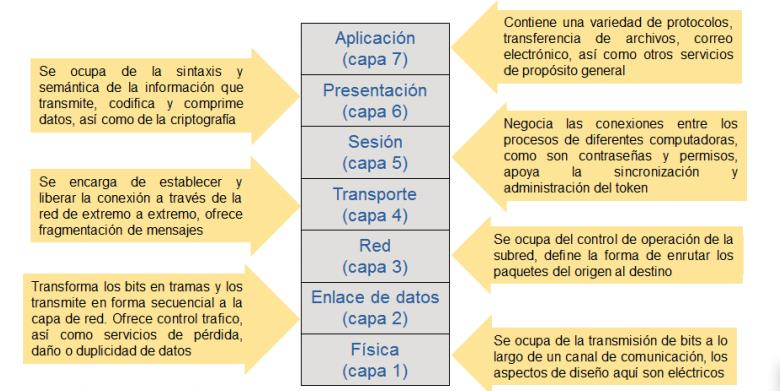
\includegraphics[scale=.7]{23.jpg}\par} \vspace{1cm}
\end{figure}
\newpage

\begin{center}
\section{\textbf{Modelo TCP / IP}}
\end{center}

\begin{figure}[h!]
		\centering
		{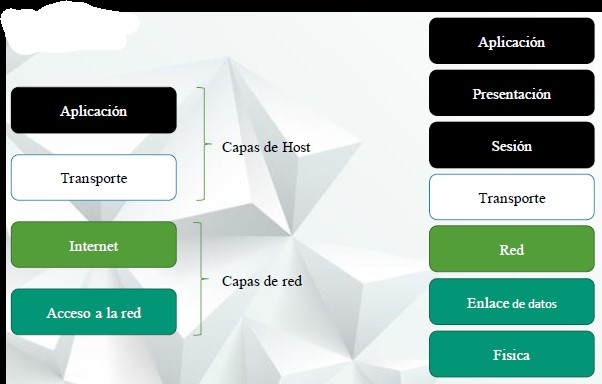
\includegraphics[scale=.7]{24.jpg}\par} \vspace{1cm}
\end{figure}

\textbf{Aplicación}: Servicio específico a usuarios y de acuerdo a la aplicación se utiliza el protocolo adecuado.\hfill \break
\textbf{Transporte}: En la capa internet no se garantiza él envió de paquetes, el orden inadecuado y tamaño pequeño de paquetes. La capa transporte realiza la transmisión de datos optima de cualquier tamaño y libre de errores el nivel de transporte se va a comprometer a segmentar en paquetes, enviarlos en un orden adecuado, ensamblar en el destino y asegurarnos que no se perdió ninguno y son correctos. Utiliza protocolos TCP y UDP.\hfill \break
\textbf{Internet}: Comportamiento de intercambio de paquetes en la red. Solo se tienen un protocolo a usar que es IP (IPv 4 o IPv 6).\hfill \break
\textbf{Acceso a la red}: No se define en el modelo, solo indica que debemos disponer de un enlace entre equipos, ya sea wifi, ethernet etc.
\newpage

{\raggedright
\subsection{Actividad 4 en clase.}
}

Realiza un ejemplo de transferencia de datos utilizando como referencia el modelo TCP / IP.

\begin{figure}[h!]
		\centering
		{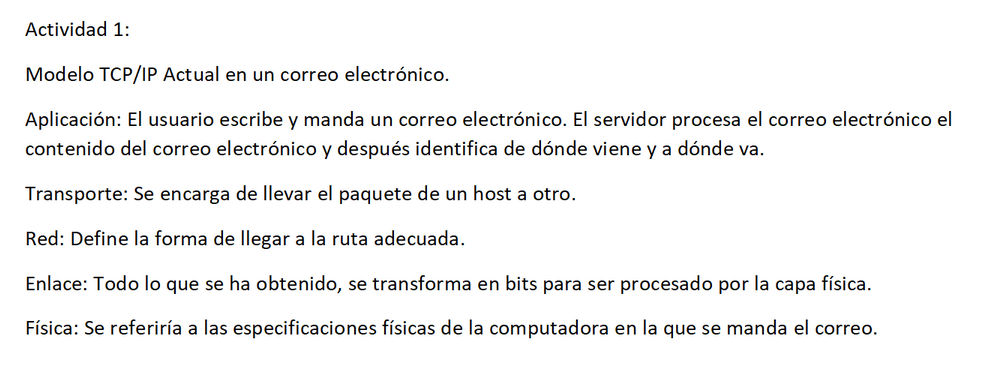
\includegraphics[scale=.8]{25.jpg}\par} 
\end{figure}

\begin{center}
\subsection{Protocolos y paquetes}
\end{center}

Protocolos son un conjunto de reglas para la interacción de procesos concurrentes en sistemas distribuidos, en diferentes campos como sistemas operativos, redes de computadoras o comunicación de datos.
Uno de los más usados es TCP/IP (Transmission Control Protocol / Internet Protocol), este conjunto tiene menor número de capas que el modelo OSI, por lo que se considera un incremento en su eficiencia.


\begin{center}
\subsection{Paradigmas de cómputo y cómo se integran en los modelos arquitectónicos de los sistemas distribuidos.}
\end{center}

La arquitectura de un sistema es su relación y estructura entre los componentes y como están relacionados. Algunos modelos arquitectónicos principales de los sistemas distribuidos son:

\begin{itemize}
	\item Paradigmas cliente - servidor
	\item Pree - to - peer
	\item Grid
	\item Proxy
	\item Cluster
\end{itemize}

{\raggedright
\subsubsection{\textbf{Modelo Cliente - Servidor}}
}

Una de las arquitecturas más citadas, los procesos toman el rol de ser clientes o servidores, los procesos de cliente interactúan con los procesos de servidor individuales en equipos de trabajo.

\begin{figure}[h!]
		\centering
		{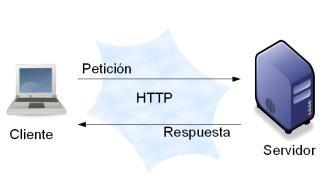
\includegraphics[scale=.7]{26.jpg}\par} \vspace{1cm}
\end{figure}

Cliente servidor para varios clientes, grupo de servidores interconectados en modelo cliente servidor.

\begin{figure}[h!]
  \begin{subfigure}
    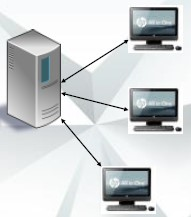
\includegraphics[scale=.6]{27.jpg}
  \end{subfigure}
  \hfill
  \begin{subfigure}
    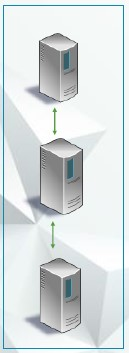
\includegraphics[scale=.5]{28.jpg}
  \end{subfigure}
\end{figure}

{\raggedright
\subsubsection{\textbf{Peep-to-peer}}
}

En el modelo cliente servidor tradicional, se tiene dos nodos que son clientes o servidores y los clientes solicitan servicios y el servidor los proporciona. Sin embargo, en los sistemas peer to peer (P2P) no se requiere una infraestructura dedicada, cada peer puede tomar el papel tanto de servidor como de cliente al mismo tiempo.

{\raggedright
Beneficios:
}

\begin{itemize}
	\item Nodos comparten recursos
	\item Se pueden desplegar algoritmos distribuidos
	\item Escalamiento más fácil del sistema
	\item Ahorro de costos
	\item Flexibilidad
	\item Ningún punto único de falla
	\item Mayor robustez del sistema
\end{itemize}

eMule mejora de eDonkey 2000 y con la colaboración de la comunidad Open.

Millones de usuarios en todo el mundo se acostumbraron a compartir y descargar archivos a través de las redes eDonkey y Kad, tras conectarse a una amplia lista de servidores.

\begin{figure}[h!]
		\centering
		{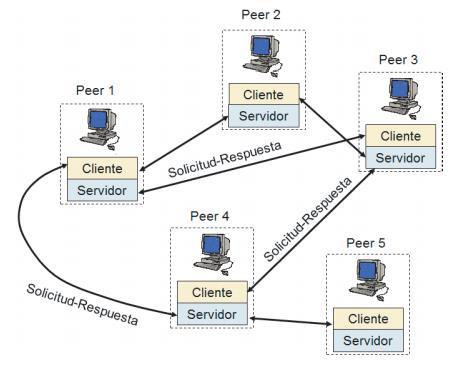
\includegraphics[scale=.7]{29.jpg}\par} \vspace{1cm}
\end{figure}

Tiene una infraestructura de comunicación par a par, se forma por grupo de nodos ubicados en una red física, estos nodos construyen una abstracción de red conocida como red superpuesta.

Una red superpuesta se establece para cada sistema P2P a través de conexiones TCP o HTTP, la red superpuesta construye túneles lógicos entre pares de nodos para implementar su propio mecanismo de enrutamiento para transportar sus mensajes.

\begin{figure}[h!]
		\centering
		{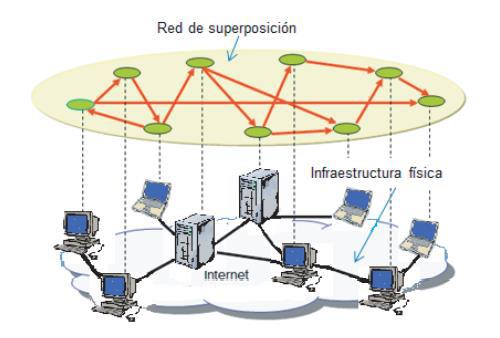
\includegraphics[scale=.9]{30.jpg}\par} \vspace{1cm}
\end{figure}

{\raggedright
\subsubsection{\textbf{Grid}}
}

Infraestructura de gestión de recursos distribuidos que se centra en el acceso coordinado a los recursos informáticos remotos. A diferencia del cómputo de clúster, el computo grid tiende a ser más heterogéneo y disperso geográficamente. Los recursos que son integrados por una infraestructura grid con plataformas de cómputo dedicadas a super computadoras de alta gama o clúster de propósito general.

Beneficios del cómputo Grid

\begin{itemize}
	\item Explotación de recursos infrautilizados
	\item Capacidad de CPU paralelos
	\item Recursos virtuales y organizaciones virtuales
	\item Acceso a recursos adicionales
	\item Balanceo de recursos
	\item Fiabilidad
	\item Mejora en gestión de infraestructura de TI distribuidos
\end{itemize}

\begin{figure}[h!]
		\centering
		{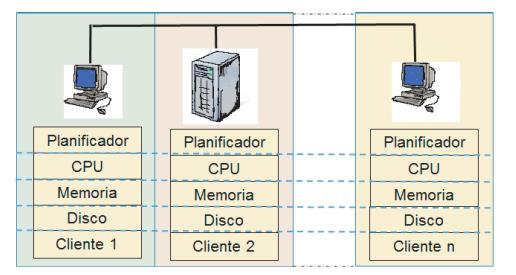
\includegraphics[scale=.7]{31.jpg}\par} \vspace{1cm}
\end{figure}

{\raggedright
\subsubsection{\textbf{Proxy }}
}

Es un servidor que se emplea como intermediario entre las peticiones de recursos que realiza un cliente a otro servidor.

Computadora A solicita un recurso a la computadora C, realizará la petición a la computadora B, que a su vez trasladará la petición a la computadora C, con lo cual la computadora C no sabrá que la petición fue de la computadora A.

Esto se usa para soportar:

\begin{itemize}
	\item Proporcionar caché
	\item Control de acceso
	\item Registro del tráfico
	\item Prohibir cierto tipo de tráfico
	\item Mejorar el rendimiento
	\item Mantener el anonimato
\end{itemize}

El proxi más conocido es el servidor proxy web, su función principal es interceptar la navegación de los clientes por páginas web por motivos de seguridad, rendimiento, anonimato, etc.

\begin{figure}[h!]
		\centering
		{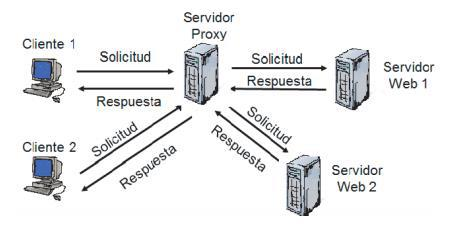
\includegraphics[scale=.7]{32.jpg}\par} \vspace{1cm}
\end{figure}

{\raggedright
\subsubsection{\textbf{Clúster}}
}

Conjuntos de computadoras construidos mediante el uso de hardware común y se comportan como si fueran una única computadora. Uso de clústeres va desde aplicaciones de super cómputo, servidores web y comercio electrónico hasta software de misiones críticas y bases de datos de alto rendimiento.

Servicios de un clúster:

\begin{itemize}
	\item Alto rendimiento
	\item Alta disponibilidad
	\item Escalabilidad
	\item Balanceo de carga
\end{itemize}

Tipos de clúster:

\begin{itemize}
	\item \textbf{Clúster homogéneo}: Cuando todas las computadoras tienen la misma configuración en hardware y sistema operativo.
	\item \textbf{Clúster semihomogéneo}: Cuando las computadoras tienen diferente rendimiento, pero guardan una similitud con respecto a su arquitectura y sistema operativo.
	\item \textbf{Clúster heterogéneo}: Cuando las computadoras tienen diferente hardware y sistema operativo.
\end{itemize}

\begin{figure}[h!]
		\centering
		{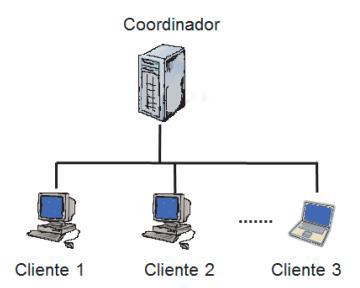
\includegraphics[scale=.9]{33.jpg}\par} \vspace{1cm}
\end{figure}

{\raggedright
\subsubsection{\textbf{Applets}}
}

Un applet es un código que se ejecuta en el contexto de otro programa, como un navegador Web, el código se descarga en el navegador y se ejecuta allí. Un applet carece de uso independiente y son muy utilizados en aplicaciones móviles, los applets no sufren los retrasos o variabilidad de ancho de banda, aunque un applet tiene privilegios restringidos de seguridad, no tiene acceso al sistema de archivos local. Un applet es no confiable a menos que lleve una firma digital de una entidad especificada como confiable.\hfill \break

Ejemplos de los applets más comunes son:

\begin{itemize}
	\item Java applets
	\item Animaciones Flash
	\item Windows media player
	\item Modelos 3D
\end{itemize}

Los applets son considerados algo en desuso, sin embargo Oracle considera que aunque su uso sea bajo, siempre es interesante ver con ejemplos sus posibilidades técnicas y aprender de ellas.

\begin{itemize}
	\item Funciones especializadas, como por ejemplo, applets para calcular el valor del ángulo inscrito en una circunferencia y circuncentro de un triángulo.
	\item Mostrar efectos visuales e imágenes con sonidos y agregar efectos sonoros.
	\item Gráficos interactivos, reaccionando a acciones que se toman con el mouse sobre el gráfico.
	\item Crear diagramas y gráficas, como por ejemplo, la clásica gráfica de trozos de pastel.
	\item Juegos sencillos.
\end{itemize}

\begin{center}
\subsection{Arquitectura de capas}
\end{center}

Un sistema complejo puede ser dividido en capas, las capas superiores hacen uso de los servicios ofrecidos por las capas inferiores. Para los sistemas distribuidos, los servicios se organizan de una manera vertical como capas de servicio, un servicio puede ser proporcionado por uno o más procesos del servidor y con los procesos de cliente se mantiene una visión de todo el sistema.\hfill \break

Ejemplo:

Ajustar la hora entre los clientes, puede realizarse por un servicio de hora de red a través de internet, usando el protocolo de tiempo de red (NTP).

\begin{figure}[h!]
		\centering
		{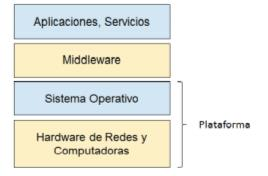
\includegraphics[scale=1]{34.jpg}\par} \vspace{1cm}
\end{figure}

{\raggedright
\subsection{Sistema distribuido se constituye por:}
}

1. Plataforma

2. Middleware

3. Aplicaciones y servicios\hfill \break

\textbf{Plataforma: }Se compone de las capas de hardware y software de nivel más bajo, son implementadas de manera independiente en cada equipo, conduciendo a la interfaz de programación del sistema hasta un nivel que facilita la comunicación y la coordinación entre los procesos.

\textbf{Middleware}: Es un software que tiene como función proporcionar un modelo de programación conveniente a los programadores de aplicaciones.

Ejemplos de middleware: 

\begin{itemize}
	\item CORBA
	\item JAVA
	\item RMI
\end{itemize}

\textbf{Aplicaciones y servicios:} Prestaciones que ofrece el sistema distribuido a los usuarios aplicaciones distribuidas.

\begin{center}
\subsection{Middleware}
\end{center}

Son representados por estándares como ODBC, OLE, DCOM y CORBA, permite distribuir datos y procesos a través de un sistema multitarea, una red local, una red remota o internet, los servicios de middleware se clasifican como:

\begin{itemize}
	\item Servicios de desarrollo
	\item Servicios de administración
\end{itemize}

Un objetivo principal es la transparencia en los sistemas distribuidos por medio de:

\begin{itemize}
	\item Ofrecer la capacidad, así como solicitar y recibir de manera transparente al sistema.
	\item Liberar a los diseñadores y administradores del sistema de problemas derivados por la complejidad del sistema operativo.
\end{itemize}

Middleware es representado por procesos u objetos en un conjunto de equipos que interactúan entre sí para implementar la comunicación de equipos que interactúan entre sí para implementar la comunicación y el intercambio de recursos de soporte para las aplicaciones distribuidas. Para conservar la transparencia se desarrolla diversas versiones de un sistema middleware, donde cada versión sea confeccionada para una clase especifica de aplicaciones.

\begin{figure}[h!]
		\centering
		{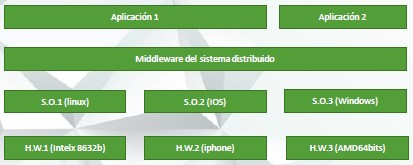
\includegraphics[scale=.9]{35.jpg}\par} \vspace{1cm}
\end{figure}

\begin{figure}[h!]
		\centering
		{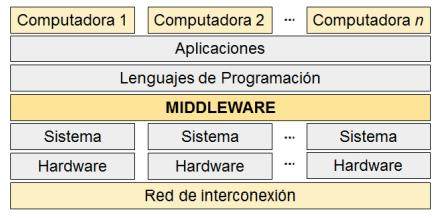
\includegraphics[scale=1]{36.jpg}\par} \vspace{1cm}
\end{figure}

Los middlewares basados en componentes permiten ocultar detalles de bajo nivel asociados al middleware, gestión de las complejidades de establecer aplicaciones distribuidas con propiedades no funcionales apropiadas como la seguridad y el apoyo apropiado de estrategias de implementación.

Los middlewares basados en objetos distribuidos proporcionan un modelo de programación basado en principios orientada a objetos y lleva los beneficios del enfoque. Principales ejemplos de middleware basado en objetos distribuidos son Java RMI y CORBA.

\begin{center}
\subsection{Corba}
\end{center}

Es una herramienta middleware que facilita el desarrollo de aplicaciones distribuidas en entornos heterogéneos tanto en hardware como en software.\hfill \break

Ejemplos:

\begin{itemize}
	\item Distintos sistemas operativos (Unix, Windows, MacOs, etc.)
	\item Distintos protocolos de comunicación (TCP/ IPX, IPX, etc.)
	\item Distintos lenguajes de programación (java, C, C++, etc.)
	\item Distinto hardware
\end{itemize}

